\documentclass[]{guo}
\usepackage{guo}
\usepackage{minted}
\usepackage{titlesec}
\usepackage{indentfirst}
\usepackage[epsilon]{backnaur}
\usepackage[labelformat=empty]{caption}

% source code listing
\usemintedstyle{vs}

% title
\titleformat
{\section}
[block]
{\fontlf}
{}
{0ex}
{}
[]
\setcounter{section}{0}

\titleformat
{\subsection}
[block]
{\fontli}
{}
{0ex}
{}
[]
\setcounter{subsection}{0}

\titleformat
{\subsubsection}
[block]
{\fontlj}
{}
{0ex}
{}
[]
\setcounter{subsubsection}{0}

% figure
\renewcommand{\figurename}{}
\renewcommand{\thefigure}{}

\begin{document}

% \papertitle{编译原理实验报告}
\paperauthor{何柏超}
\studentno{3112005816}
\colleage{计算机学院}
\major{计算机科学与技术}
\grade{2012}
\class{2}
\supervisor{张三}

% Badge
\begin{flushleft}
    \hspace{8.5mm}
    
\includegraphics[height=2.19cm,width=2.21cm]{resource/badge.jpg}
\end{flushleft}

% School Brand
\begin{center}
    
\includegraphics[height=2.96cm,width=10.56cm]{resource/brand.jpg}
\end{center}
\vspace{6.5mm}

% Paper Title
\begin{center}
    {\fonthei\bfseries\fontla{\papertitle{}}}
\end{center}
\vspace{20mm}

% Paper Meta
\begin{center}
    \makeatletter

    {\fonthei\fontlg{%
            学\hspace{2em}院\hspace{3mm}\drawunderline{\colleage{}}
            \\ \vspace{2.4mm}
    }}
    {\fonthei\fontlg{%
            专\hspace{2em}业\hspace{3mm}\drawunderline{\major{}}
            \\ \vspace{2.4mm}
    }}
    {\fonthei\fontlg{%
            年级班别\hspace{3mm}\drawunderline{\grade{} 级(\class{})班}
            \\ \vspace{2.4mm}
    }}
    {\fonthei\fontlg{%
            学\hspace{2em}号\hspace{3mm}\drawunderline{\studentno{}}
            \\ \vspace{2.4mm}
    }}
    {\fonthei\fontlg{%
            学生姓名\hspace{3mm}\drawunderline{\paperauthor{}}
            \\ \vspace{2.4mm}
    }}
    {\fonthei\fontlg{%
            指导教师\hspace{3mm}\drawunderline{\supervisor{}}
            \\ \vspace{2.4mm}
    }}

    \makeatother
\end{center}
\vfill

\begin{center}
    \makeatother
    {\fontlg\fonthei{2014 年 12 月}}
    \makeatother
\end{center}


\section{一、实验目的与要求}

目的:通过对提供的 PL/0 编译程序进行研究、学习,在该程序的基础上对其
词法分析程序、语法分析程序和语义处理程序进行修改和拓展;
从而深入了解编译原理的基本原理和基本实现方法。


要求:对 PL/0 做以下修改扩充:

\begin{enumerate}
    \item[(1)] 增加单词:
        \begin{itemize}
            \item 保留字:\mintinline{pascal}{ELSE},\mintinline{pascal}{FOR},\mintinline{pascal}{STEP},\mintinline{pascal}{DO},\mintinline{pascal}{RETURN}
            \item 运算符:\mintinline{c}{*=},\mintinline{c}{/=},\mintinline{c}{&&},\mintinline{c}{||},\mintinline{c}{!}
        \end{itemize}
    \item[(2)] 修改单词: 不等号 $\#$ 改为 $<>$
    \item[(3)] 增加条件语句的 \mintinline{pascal}{ELSE} 子句,要求:给出相关文法、语法描述图、语义描述图。
\end{enumerate}

\section{二、实验环境与工具}

\begin{enumerate}
    \item[(1)] 计算机及操作系统: PC 机,Windows XP / Windows 7
    \item[(2)] 程序设计语言: C / C++
    \item[(3)] 使用软件: Borland C++ Builder 6
    \item[(4)] 教学型编译程序: PL/0
\end{enumerate}

\section{三、开发过程及完成情况}

\subsection{1. 增加单词}

本实验总共新增 5 个关键字和添加 5 个运算符。
首先需要为这几个单词添加对应的 \mintinline{c}{SYMBOL} 常量:

\begin{table}[H]
    \centering
    \begin{tabular}{l c}
        ELSE & \mintinline{c}{SYM_ELSE} \\
        FOR & \mintinline{c}{SYM_FOR} \\
        STEP & \mintinline{c}{SYM_STEP} \\
        DO & \mintinline{c}{SYM_DO} \\
        RETURN & \mintinline{c}{SYM_RETURN} \\
        *= & \mintinline{c}{SYM_MUL_ASSIGN} \\
        /= & \mintinline{c}{SYM_DIV_ASSIGN} \\
        \&\& & \mintinline{c}{SYM_AND} \\
        || & \mintinline{c}{SYM_OR} \\
        ! & \mintinline{c}{SYM_NOT} \\
    \end{tabular}
\end{table}

\inputminted[baselinestretch=0.75,firstline=82,lastline=100,fontsize=\fontlm]{cpp}{Unit1.cpp}

为了能够让词法分析程序正确识别到对应的token,我们需要在 \mintinline{c}{GetSym}
函数中添加对应的识别过程。

其中 \mintinline{c}{!} 是单字母 token,所以直接在 \mintinline{c}{ASCII_SYMBOL}
数组中添加即可。

\inputminted[baselinestretch=0.75,firstline=2496,lastline=2497,fontsize=\fontlm]{cpp}{Unit1.cpp}

对于保留字 token,我们只要将其按照字典序升序加入\mintinline{c}{KW_SYMBOL}数组
即可在 \mintinline{c}{GetSym} 函数中被识别出来:

\inputminted[baselinestretch=0.75,firstline=2526,lastline=2537,fontsize=\fontlm]{cpp}{Unit1.cpp}

而由于多字符的运算符中包含一些和一个字母的运算符相同的前缀,
所以我们要进行超前查看一个字符来判断属于何种类型的 SYMBOL:

\inputminted[baselinestretch=0.75,firstline=514,lastline=522,fontsize=\fontlm]{cpp}{Unit1.cpp}
\inputminted[baselinestretch=0.75,firstline=586,lastline=595,fontsize=\fontlm]{cpp}{Unit1.cpp}

通过修改以上几个地方,我们就可以试编译程序成功识别到新增加的单词:

\begin{figure}[h!]
    \caption{新增加的关键字}
    \centering
        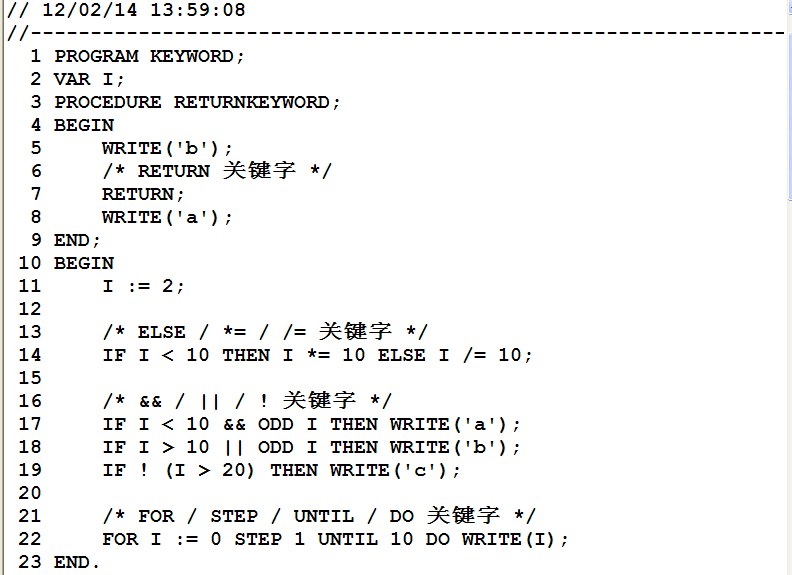
\includegraphics[scale=0.5]{figure/keywords.png}
\end{figure}

\clearpage

\begin{figure}[h!]
    \caption{新增加的关键字程序运行截图}
    \centering
        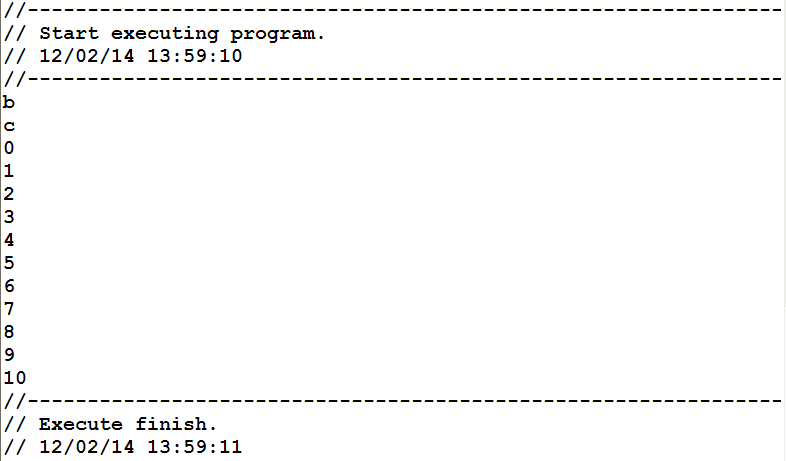
\includegraphics[scale=0.25]{figure/keywords-output.png}
\end{figure}

从截图上我们可以看到编译程序已经可以正确执行对应的新增关键字代码,
这需要我们添加对应的递归子程序实现:

\inputminted[baselinestretch=0.75,firstline=1277,lastline=1304,fontsize=\fontlm]{cpp}{Unit1.cpp}


至此我们已经完成了添加新关键字的功能。

\clearpage

\subsection{2. 修改单词}

因为本实验需要把一个字符的运算符改成两个字符的运算符,
所以我们需要将其从 \mintinline{c}{ASCII_TABLE} 数组中移除,
并在 \mintinline{c}{GetSym} 函数中添加对应的识别判断:

\inputminted[baselinestretch=0.75,firstline=562,lastline=573,fontsize=\fontlm]{cpp}{Unit1.cpp}

这样就可以修改不等号为\mintinline{c}{<>}的形式了:

\begin{figure}[h!]
    \caption{修改不等号的测试程序}
    \centering
        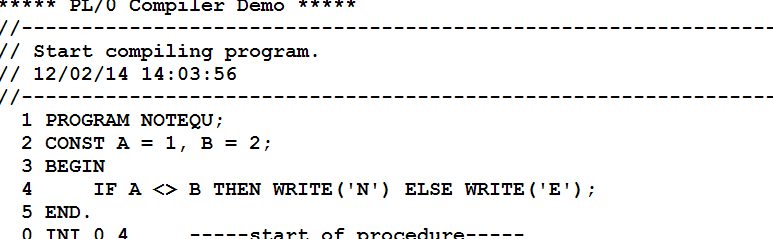
\includegraphics[scale=0.5]{figure/not_equ.png}
\end{figure}

\begin{figure}[h!]
    \caption{修改后的运行结果}
    \centering
        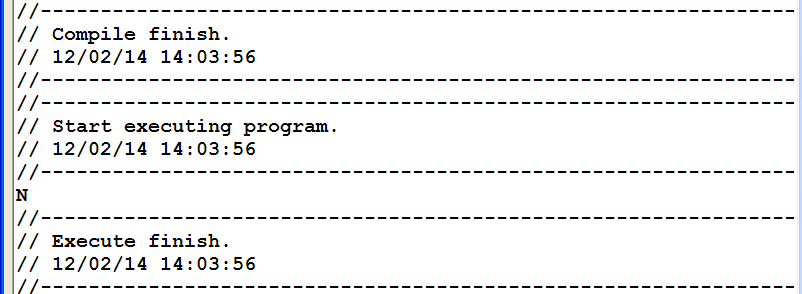
\includegraphics[scale=0.25]{figure/not_equ-output.png}
\end{figure}

\clearpage

\subsection{3. 增加 \mintinline{pascal}{ELSE} 子句}

\subsubsection{文法:}
\begin{bnf*}
    \bnfprod{IF-STMT}
        {\bnfts{IF} \bnfpn{EXPRESSION} \bnfts{THEN} \bnfpn{STATMENT} \bnfpn{ELSE-CLAUSE}}\\
    \bnfprod{ELSE-CLAUSE}
        {\bnfts{ELSE} \bnfpn{STATMENT} \bnfor \bnfes}
\end{bnf*}

\subsubsection{语法描述图:}
{\centering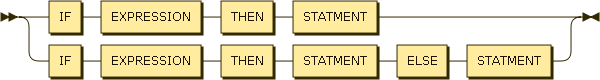
\includegraphics[scale=0.75]{figure/if-stmt-railroad.png}}

\subsubsection{语义描述:}

为了方便描述,我们将上述文法改写成如下:

\begin{bnf*}
    \bnfprod{S}
        {\bnfpn{E} \bnfpn{S1}}\\
    \bnfprod{S}
        {\bnfpn{E} \bnfpn{S1} \bnfpn{S2}}\\
\end{bnf*}

\begin{table}[H]
    \centering
    \begin{tabular}{l p{10cm}}
        $S \rightarrow E \ S1$ & backpatch(E.truelist, S1.quad); \newline
                                 S.nextlist = merge(E.falselist, S1.nextlist) \\
        $S \rightarrow E \ S1 \ S2$ & backpatch(E.truelist, S1.quad); \newline
                                      backpatch(E.falselist, S2.quad); \newline
                                      S.nextlist = merge(E.falselist, S1.nextlist, S2.nextlist);
    \end{tabular}
\end{table}

\subsubsection{实现:}

为了实现对 ELSE 子句的解析,我们需要改写 \mintinline{c}{parse_if} 函数。

首先我们要在条件判断之后添加一个 false jump 指令来实现当条件不满足时跳过 THEN 子句:

\inputminted[baselinestretch=0.75,firstline=1822,lastline=1824,fontsize=\fontlm]{cpp}{Unit1.cpp}

在解析 THEN 子句之后,我们需要超前查看一个 token 来判断是否存在 ELSE 子句,
如果存在,则需要生成一条无条件跳转指令来跳过 ELSE 子句:

\inputminted[baselinestretch=0.75,firstline=1826,lastline=1842,fontsize=\fontlm]{cpp}{Unit1.cpp}

注意到我们在解析 THEN 子句的指令后会对先前生成 false jump 指令进行回填:

\inputminted[baselinestretch=0.75,firstline=1837,lastline=1837,fontsize=\fontlm]{cpp}{Unit1.cpp}

以及在解析 ELSE 子句后会对 THEN 子句最后的无条件跳转子句进行回填:

\inputminted[baselinestretch=0.75,firstline=1839,lastline=1839,fontsize=\fontlm]{cpp}{Unit1.cpp}

通过上述的改写我们即可以正确解析带有 ELSE 子句的测试程序:

\begin{figure}[h!]
    \caption{带有 ELSE 子句的测试程序}
    \centering
        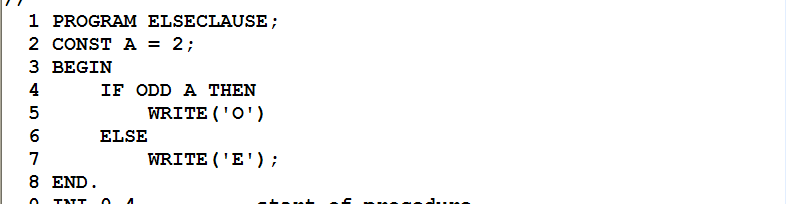
\includegraphics[scale=0.5]{figure/else_clause.png}
\end{figure}

\begin{figure}[h!]
    \caption{程序运行结果}
    \centering
        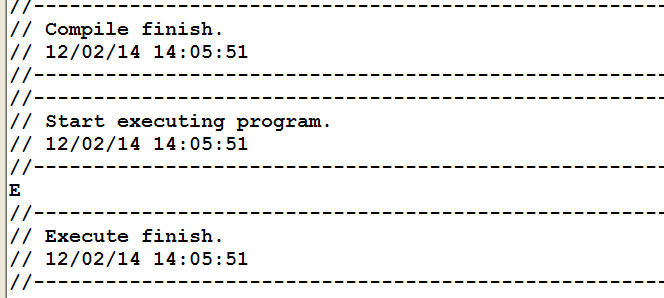
\includegraphics[scale=0.4]{figure/else_clause-output.png}
\end{figure}

\clearpage

\section{四、心得体会}

通过这三个实验,加深了我对 PL/0 编译程序的理解;让我有机会把课程上学习到的知识
应用到实践中。通过这几个不同方面的功能改造,为后面的课程设计工作打下了基础。


\end{document}
